
\section{Array, CTE, Tree, XML, JSON, Graph, hstore}

\begin{breakbox}
\boxtitle{Create Table With Array:}
\sql{sql_code/array_create_table.sql}

%\begin{lstlisting}[language=SQL,aboveskip=1pt, belowskip=2pt]
%SELECT ARRAY[1,2,3+4];
%\end{lstlisting}
\end{breakbox}

\begin{breakbox}
\boxtitle{Array Insert:}
\sql{sql_code/array_insert.sql}
\end{breakbox}

\begin{breakbox}
\boxtitle{Array Constructors:}
\sql{sql_code/array_constructors.sql}
\end{breakbox}

\begin{breakbox}
\boxtitle{Array Select:}
\sql{sql_code/array_select.sql}
\end{breakbox}

\begin{breakbox}
\boxtitle{Array Operators:}
\sql{sql_code/array_operators.sql}
\end{breakbox}

\begin{breakbox}
\boxtitle{Array Functions:}
\sql{sql_code/array_functions.sql}

Further: not equal <>, comparison < =< > >= (lexicographical comparison of elements), contains @>, array-to-array concatenation ||.
\end{breakbox}

\begin{breakbox}
\boxtitle{CTE:}

Temporary, named result set. Can be referenced later and has recursion unlike a nested statement. Execution scope of a SELECT, INSERT, UPDATE, or DELETE statement.

\sql{sql_code/cte_non_recursive.sql}

\sql{sql_code/cte_recursive.sql}
\end{breakbox}

\begin{breakbox}
\boxtitle{Tree Data Structures:}

Given:
\begin{center}
	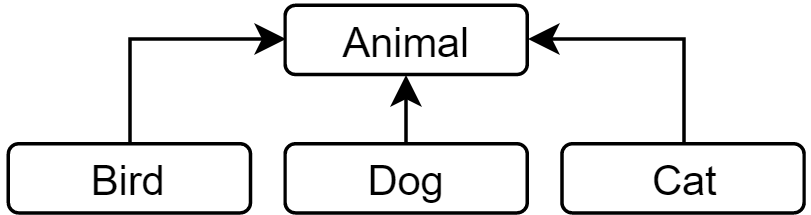
\includegraphics[width=.10\textwidth]{slides_images/tree_given_example}
\end{center}

\textbf{Adjacency list:}

\begin{tabular}{lll}
id & name   & parent\_id \\
\hline
1  & Animal & NULL       \\
2  & Bird   & 1          \\
3  & Dog    & 1          \\
4  & Cat    & 1         
\end{tabular}

\textbf{Nested Set:}
\begin{center}
	\includegraphics[width=.13\textwidth]{slides_images/trees_nested_set}
\end{center}

\begin{tabular}{llll}
id & name   & left & right \\
\hline
1  & Animal & 1    & 8     \\
2  & Bird   & 2    & 3     \\
3  & Dog    & 4    & 5     \\
4  & Cat    & 6    & 7    
\end{tabular}

\textbf{Materialised Path:}

\begin{tabular}{lll}
id & name   & lineage (e.g. ltree, array or string) \\
\hline
1  & Animal & 1                    \\
2  & Bird   & 1,2                  \\
3  & Dog    & 1,3                  \\
4  & Cat    & 1,4                 
\end{tabular}
\end{breakbox}

\begin{breakbox}
\boxtitle{XML:}

\begin{itemize}
	\item \textbf{XPath:} Extract/filter
	\item \textbf{XQuery:} Querying, uses XPath syntax
\end{itemize}

To convert a table to XML:
\sql{sql_code/xml_table_to_xml.sql}

\sql{sql_code/xml_students.sql}
\end{breakbox}

\begin{breakbox}
\boxtitle{JSON/JSONB:}

Typical JSON document, can be nested (see address):
\sql{sql_code/json_person_example.sql}

\textbf{JSONB} (binary) has no duplicate keys and last key wins. Postgres uses a hashing function to store them in binary. Keys are sorted.
\sql{sql_code/json_jsonb_example.sql}

\textbf{Operators:}
\sql{sql_code/json_operators.sql}

\textbf{Functions:}
	\begin{itemize}
		\item array\_to\_json(anyarray), row\_to\_json(record), to\_json(anyelement), json\_array\_length(json)
		\item json\_object\_keys(json), json\_array\_elements(json) expands a JSON array to a set of JSON elements
	\end{itemize}
\end{breakbox}

\begin{breakbox}
\boxtitle{Traversing Graph With CTE:}
\sql{sql_code/cte_graph_traversal.sql}
\end{breakbox}

\begin{breakbox}
\boxtitle{Key Value Pairs (hstore):}

''RDBMS are designed for consistency and efficiency. By using KVP schema you throw the retrieval capability down the drain!''

Possibly suitable for
\begin{itemize}
	\item Easy data storage and data capture
	\item Rows with many attributes that are rarely examined
	\item Semi-structured data
\end{itemize}

\sql{sql_code/hstore_examples.sql}
\end{breakbox}